\section{Design}
\label{sec:design}

% XXX: epidemic: too general, anti-entropy
% more tech details

\begin{figure}
\centering
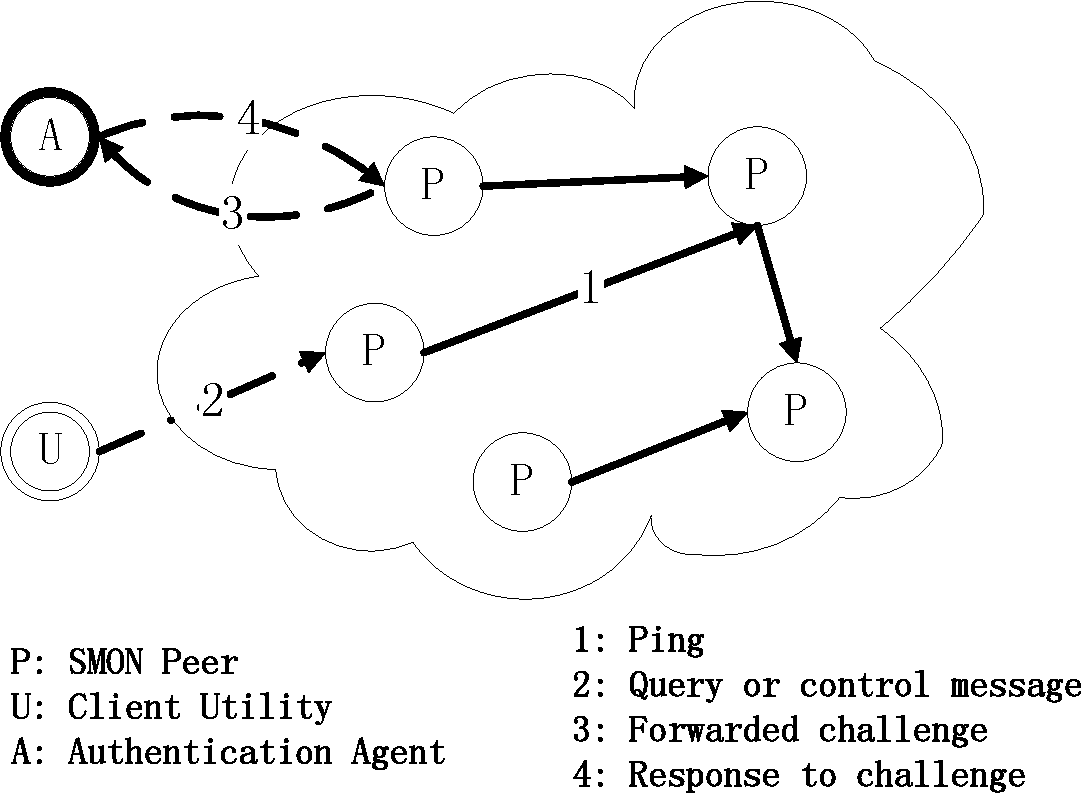
\includegraphics[width=3.0in]{smon_arch}
\caption{SMON system design. SMON peers monitor each
other by sending ping messages. User can send query or control messages
to any peer. Authentication agent resolves authentication
chanllenge from peers to help them login into other machines
automatically.}
\label{fig:smon_arch}
\end{figure}

The design of SMON system is presented in
figure~\ref{fig:smon_arch}.  It consists of three parts: SMON
peers, authentication agent and client utility.

The SMON peers run on a set of target machines where
distributed applications will be deployed. The peers
periodically monitor and maintain each other in their
membership list. They will deploy new peers on fresh
machines, recover failed peers and upgrade themselves to new
version. In this way, a SMON system can manage itself
automatically. With the help of authentication agent, a SMON
peer can login into remote machines in its membership list
automatically to recover failed peers or deploy new peers. A
SMON system can manage a set of distributed applications. It
defines the management semantic for long running services.
User can use the client utility to instruct SMON on
application management. The utility can also be used to
control a SMON system, such as upgrading it to new version,
or query running states of SMON peers.

The epidemic algorithm is used extensively in designing
SMON. A SMON system must hold several distributed invariants
to run successfully. For example, there should be a SMON
peer running on all target machines specified by user. The
epidemic algorithm is applied for the invariant as follows:
a SMON peer will periodically ping another random peer in
its membership list, if corresponding pong message is not
received within timeout, it will try to recover the remote
peer or deploy a new peer on the remote machine. The
epidemic algorithm is also used to hold other invariants.
% XXX: for example?

We use epidemic algorithm for several reasons. First, it has
inherent scalability. Second, the epidemic algorithm is
simple and easy to implement. By its simplicity, the SMON
system is less prone to runtime errors so that it can run
reliably for long time. Third, it is robust and resilient to
failure.

% The SMON peers run on a set of target machines where
% distributed applications will be deployed. Each peer
% maintains the full list of target machines as its membership
% list. The peers monitor and maintain each other using
% epidemic algorithm. A peer periodically chooses a random
% peer and sends it a ping message.  If the pong message is
% not replied within a timeout interval, the remote peer is
% considered as failed. The peer will try to recover the
% failed one by restarting it remotely, or deploying and
% starting a new peer on a fresh machine. Each peer has an
% associated version number. The peers exchanges their version
% numbers epidemically and peers of lower version upgrade
% themselves to the latest versions. The epidemic algorithm
% ensures that the entire SMON system will keep running and
% staying at the latest version eventually.
% 
% The authentication agent holds the credential (e.g. private
% key) used to authenticate with the target machines. When
% a SMON peer tries to deploy or restart another peer, it can
% automatically login into the remote machine with the help of
% the agent. The credential is never known to the peers or
% leaked out.
% 
% % XXX: quite basic?
% With the help of client utility, user can instruct SMON to
% manage a set of distributed applications. SMON deploys and
% maintains distributed applications using epidemic
% algorithms too. The application management semantic of SMON
% is quite basic. User can extend the management semantic by
% deploying another management system upon SMON.



\comment{
\subsection{Monitor-reaction model}

%The collective behaviour of all peers defines the runtime
%of a SMON system.

\begin{figure}
\centering
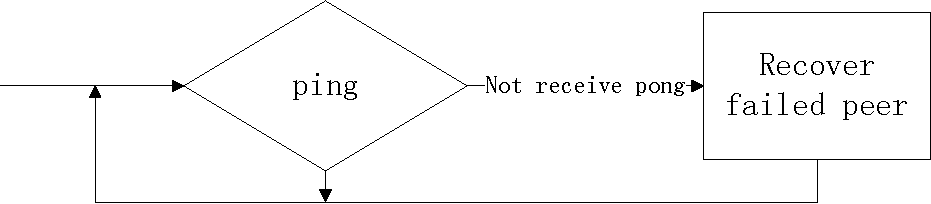
\includegraphics[width=3.0in]{recover}
\caption{recover model}
\label{fig:recover}
\end{figure}

We use a monitor-reaction model to define SMON peer's
behaviors. The model is consistent with and automatically
implements what humans do when maintaining a distributed
system manually. In the model, the ``monitor'' part defines
what status to observe timely, and based on the monitored
result, certain ``reactions'' are performed. Thus, the model
describes a closed-loop control that eliminates human
interventions. For example, a SMON peer will continually ping
other peers to see if they are running. If a pong message is
not received within a predefined timeout interval, we
consider it as failed and try to recover it by login into
the machine and restart it, otherwise, an empty reaction is
performed. The model is shown in figure~\ref{fig:recover}.

The monitor-reaction model can have varations. First, one
model can be nested in the reaction part of another model.
Using previous example, when we know that a peer is failed,
there can be another reason: the machine is crashed and
maybe replaced by a new one with the same host name. To
handle such cases, in the reaction part we need to further
detect whether the machine has a SMON peer installation, if
not, we have to deploy a copy of the peer first. The model
is shown in figure~\ref{fig:recover-nest}.

Second, two or model models can be combined for purposes
such as optimization. For example, SMON peers also exchange
their version numbers and upgrade peers with low version
automatically. This model can be combined with the failure
detector model by piggyback version number within the ping
message. Thus, we can save one RPC call. The combined model
is shown in figure~\ref{fig:combine}.

One peer may implements several models. They run
concurrently and need to be well coordinated. In the upgrade
model, after a new version is retrieved, the peer need to
start the new verison and stop itself. Before it execute the
action, other models may be running also. The upgrade model
has to wait others until all of them finish actions part.
The coordination can be implemented by using locks, and in
this case, a reader-writer lock may be more suitable.

The models are required to be stateless in the sense that
the execution of a model is independent with it previous
executions. In this way, the implementation of the model is
as simple as possbile and improves peer's reliablity.

\note{transaction? the membership list update should be
atomic.}

\note{the combined model looks complex. the reason: 1. for
optimization. 2. we have carefully examined the code and it
runs for a long time without error?}

The models can not be running infinitely. We address this
problem in subsection~\ref{subsec:livetag}.
}

\subsection{Self-management}

We describe how SMON deploys, recovers and upgrades itself
automatically.

\subsubsection*{Self-deployment}

For a list of target machines, SMON can deploy itself to all
the machines automatically. At the very beginning, there is
no SMON peer deployed and running yet. A first peer have to
be deployed and started manually. It then pings other
machines in its membership list and deploys new peers. The
new peers repeat the same ping-and-deploy process. While
there are more SMON peers deployed and running, this process
speeds up exponentially. It is proved that with probability
1 all the reachable machines can be deployed
eventually\cite{Eugster2004}.

%while 1:
%  sleep(T)
%  h = randomchoice(member\_list)
%  try:
%    ping(h)
%  except Timeout:
%    remote\_copy(h, path\_to\_installation\_package)
%    remote\_execute(h, remote\_path\_to\_installation\_package)

%The ping-and-deploy process of a SMON peer implements the
%upper part of the ping model in figure~\ref{fig:combine}.
In detail, a peer $P$ will periodically choose a random
machine $M$ from its membership list and sends a ping
message. If a pong message is not received within predefined
timeout intervals, it will start the deployment procedure on
machine $M$. $P$ first authenticates itself with $M$ and
login into $M$ with help of the authentication agent
(described in \ref{subsec:security}), then it copies an
installation package of SMON peer to $M$, starts the package
remotely and logout $M$. The installation package first
checks the integrity of itself (currently using MD5 checksum)
in case of transfer errors during remote copy, then it
installs and starts SMON peer.

There may be failures (e.g. connection corrupted, machine
crashed) at any time when peer $P$ logins
into $M$, copies and starts installation package remotely.
When failure happens, $P$ will just abort the deployment
procedure. $M$ will be chosen by another SMON peer at later
time. It is expected that a new SMON peer will be deployed
on $M$ eventually.

Because peers communicate with each other epidemically, it
is possible that two or more peers try to deploy a SMON peer
on the same machine $M$ simultaneously. This race-condition
is solved without direct coordination among peers. The
installation packages from different peers will be copied to
different directories of $M$ and they will not overwrite
each other. The execution of simultaneously started
installation packages are synchronized using OS provided
facilities (e.g. lock file). So only the first installation
process will finish and others will abort. In solving the
problem, some overhead is introduced because multiple
installation packages may be copied, which wastes network
bandwidth and storage resources. Through mathematical
analysis and evaluation in Planet-Lab platform, it
is shown that the overhead is low on most machines. Since
the size of the installation package is small (122KB), the
overhead can be considered as insignificant.

It is not easy to define when self-deployment is finished
globally. Ideally, it is finished when all the target
machines are reached and deployed with SMON peers.  However,
considering some machines may be unreachable or shutdown
from time to time, the `finished-globally' situation is
rare. Even after a machine is deployed with SMON peer, it
may crash and be replaced with a new machine with the same
host name. The peers then have to continue the
ping-and-deploy process as long as they are live and leave
the `finish' definition to user. The user can query how many
or which peers are deployed, and determine whether it is
appropriate to consider the situation as a finish.

\subsubsection*{Self-upgrade}

As a distributed system, SMON can upgrade itself to a new
version automatically. The upgrade goes online while SMON is
running. User needs not to stop SMON before upgrade.

Each SMON peer has an associated version number and it is
stored persistently in configuration file with the peer.  A
peer will exchange and compare its version with other epidemically. If
there is a difference, the peer with lower version will
retrieve the installation package from the other and upgrade
itself automatically.

% XXX limit the number of ...?
It is possible that a peer of new version is
known by many peers of old version quickly. To avoid flash
crowd, the peer of new version will limit the number of
simultaneous request for retrieving installation package.

To upgrade the whole SMON system to a new version, user only
has to upgrade one peer to the new version and all the other
SMON peers will converge to the latest version eventually.
The user can upgrade a SMON peer by using the client
utility described in subsection~\ref{subsec:client}.

\comment{
\note{need revise the method, consider the ping interval}
When a SMON peer knows there's a new version of peer, a list of
hosts on which peers with new version are running is gathered
through active detection among peers.  A self-upgrade action is
scheduled to read the list and download the new version. At the
beginning of the self-upgrade process, there would only be a
small number of peers running in new version, but they are known
by a lot of other peers.  If there's not any constraints, a lot
of peers may download from the same host simultaneously. To
prevent that, we use a conservative strategy to control the
self-upgrade action.  The destination is, at average, only a
constant $k$ of peers can download simultaneously from a host.
The algorithm we use does not need any coordination among peers,
and works as follows.  If there are $n$ peers want to download
from the same host. Each of them choose to take the download
action  with probability $k/n$. If the action is not taken, it
will be delayed in the next time. So at average, there will be
only $k$ peers downloading from the same host simultaneously,
and it takes a peer to rerun the action $n/k$ times to select
the same peer.  As peers don't coordinate with each other, they
make a conservative estimation that set $n$ to $N$, the number
of all the peers. The strategy may cause a slow start at the
begin of self-upgrade process because $n$ is far smaller that
$N$. When more peers are upgraded to new version, the upgrade
process would be boosted. If a peer knows $p$ peers of new
version, the probability it choose to not download from any of
them is $q=(1-k/n)^p$ and it takes at average $\frac{1}{1-q}$
tries to choose a host. When $p$ increases, $q$ decreases
quickly and $\frac{1}{1-q}$ will be nearly 1 with large $p$.
}

\comment{
It is important to ensure that communication interfaces for
different versions of SMON peers are consistent. If the condition
is ensured, the whole SMON system can be updated gracefully while
most of peers are running and the system functions well.
Otherwise, the new SMON system can only be deployed after the old
one is stopped.
}

\subsubsection*{Self-recovery}

Two kinds of failures may happen and must be handled by
SMON, namely, machine failure and network partition.

When a machine fails, the SMON peer running on it is stopped
also. Other peers know this event through epidemic pings and
they will try to recover the failed peer by restarting it
remotely, with help from authentication agent. It is safe to
start multiple instances of SMON peer, but it is idempotent
to start only one instance.

XXX: crash-only design

Network partitions can also be handled by SMON easily. When
network partition occurs, SMON peers are splitted into
several sub-systems, each of which is connected internally.
Implied by epidemic algorithm, each partitioned part will
eventually converges to the consistent state regarding to
the version of SMON peers. When two partitions rejoin, the
peers in different part will be able to contact and
communicate with each other, leading to the mergence of
the whole system.

% In this way, a peer can choose which action to take based
% on result of a ping message.

\comment{
The SMON system has a global state indicating it is active
or not. When SMON is active, the peer-monitoring component
is enabled. Every SMON peers actively monitor each others
and keep them running as possible as they can. While SMON is
not active, the peer-monitoring function is disable and SMON
acts just like an usual management tools. The active state
is an essential part of SMON system design. Without it, SMON
is just another usual management tool for distributed
applications. If the state is designed as active all the
time, it is a hard problem to stop an active SMON system. If
we try to stop the SMON peers one-by-one, we will noticed
that the stopped peers will soon be restarted by other
peers. And the only way to stop an active SMON system is to
stop all the peers near simultaneously, which is quite hard.
The active state also has an associated version number and
each SMON peer replicates and stores the state with version
locally.  The epidemic algorithm is used to maintain the
state consistently and efficiently among all peers.
}

\subsubsection*{Disable/enable self-management}
\label{subsec:livetag}

We need mechanism to enable or disable self-management
capability of SMON to stop it from running. When
self-management is enabled, we cannot stop SMON by shutdown
peers individually.  If a peer is stopped by user, it will
be started soon by another peer. The only solution under
such condition is to stop all the SMON peers simultaneously,
which is not feasible at large scale.

We use a boolean variable called \texttt{livetag} to control epidemic
monitoring among peers. If the value is false, a peer will
stop sending periodic ping message to others and the whole
SMON system stops maintaining itself. 
%We can now stop SMON peers one by one.

The \texttt{livetag} variable has an associated version
number and is maintained on each peer distributedly. The
peers exchange \texttt{$<$livetag, version$>$} tuples
epidemically and update the tuple to the latest version.
Note that even the epidemic update of \texttt{livetag} is
controlled by the value of \texttt{livetag}.  When
\texttt{livetag} is false, peers still respond
to incoming messages, so as to
help disseminating the update to \texttt{livetag}.

Suggested by epidemic algorithm, the whole SMON system will
be finally disabled when the \texttt{livetag} value of any
peer is set to false and peers will not send ping messages
to each other. A peer will stop itself from running if no
messages is received for enough long time. In this way, a
SMON system can be shutdown automatically by setting
\texttt{livetag} to false.

\subsubsection*{Combine them together}

A SMON peer monitors and maintains other ones by combining
above-mentioned activities together.  Two points are
worth mentioning. First, as an optimization, the version
number of SMON is piggybacked in ping/pong messages among
peers.  Second, when peer $A$ considers another one $B$ as
failed, there are two possible reasons: no SMON peer is
deployed or $B$ is stopped. $A$ will restart $B$ directly
if it is already installed. 

%\note{the complete execution of a peer}

%\note{peer and installation package, how they coordinate
%when upgrade and deploy.}

%\note{the set of states peer maintains, database?,
%stateless?}


\subsection{Security mechanism}
\label{subsec:security}

SMON should have security mechanism to achieve two goals:

\begin{itemize}

  \item Help peers to authenticate with remote machines
  automatically so as to copy installation packages and
  execute commands remotely.

  \item Authenticate and encrypt access to SMON peers so it
  will not be misused (e.g. deploying malwares).

\end{itemize}

%SMON peer should be able to login into remote machines
%automatically to deploy new peers or restart failed ones.
%In this process, the authentication credential should be
%keep secret.  \note{here.} It is necessary for different
%SMON peers to authenticate each others and keep the
%communication confidential among them. In addition, when a
%SMON peer deploys new SMON peer on a remote machine, it need
%to authenticate itself with the remote machine to copy
%contents and execute commands (start the installation
%package). The authentication credential is owned by user and
%should be protected confidentially. From another point of
%view, the SMON peers relies upon the authentication
%credentials provided by user to deploy and maintain each
%others automatically in a distributed approach.

We describe how we design security mechanisms to achieve the
two goals on Planet-Lab platform and explain how to apply
the mechanisms on other distributed platforms.  Planet-Lab
uses public-key system to authenticate access to the
platform. A user access his slice (a set of distributed
virtual machines) by using ssh. The private key is kept in
user's computer and the public key is distributed to all
virtual machines of his slice.

%SMON system is designed for distributed platforms that are
%semi-open---like Planet-Lab or grid, or for proprietary
%ones---such as large machine rooms or data centers. It
%assumes that: 1) the network between machines in a
%distributed infrastructure is not trusted, 2) the users that
%can access the infrastructures are not adversarial, 3) the
%applications running in the infrastructures are not
%adversarial. Based on assumptions above, SMON designed an
%security mechanism which guarantees that 1) communications
%among SMON peers are authenticated and confidential, 2)
%authentication credentials are never leaked. The mechanism
%incorporated in current design supports challenge based
%authentications like public-key authentication scheme, which
%is extensively used.

\begin{figure}
\centering
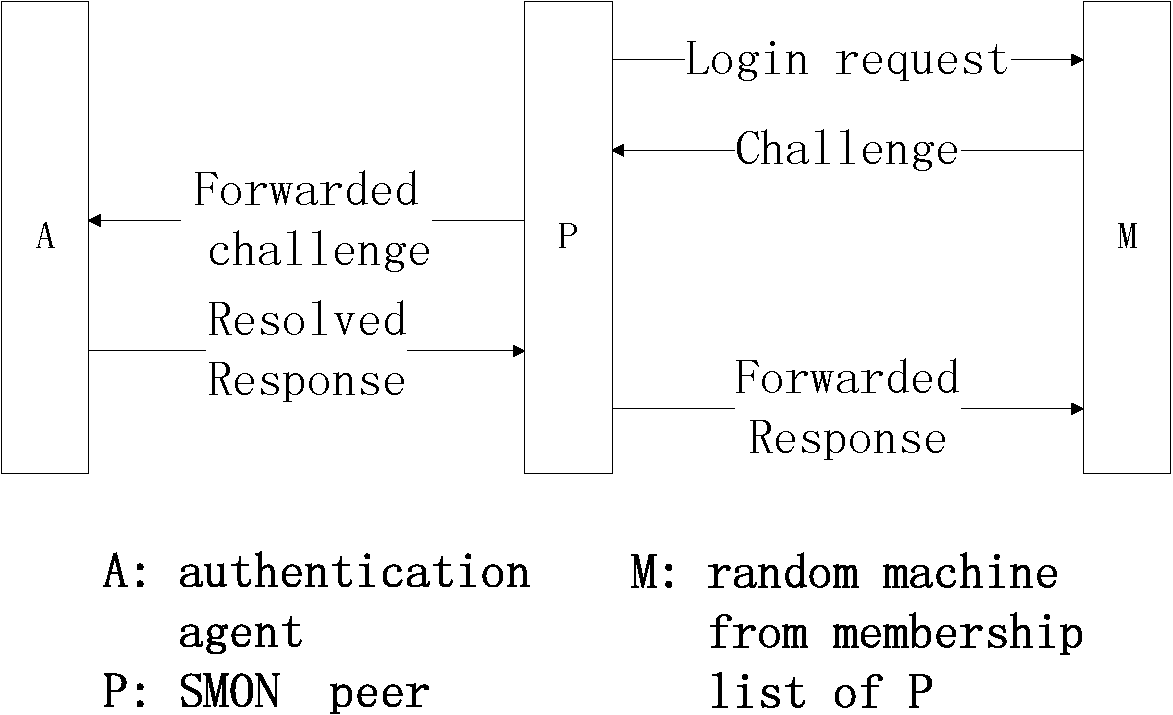
\includegraphics[width=3.0in]{auth}
\caption{Interactions among SMON peer, authentication agent
and a remote machine when the peer login into the machine.}
\label{fig:auth}
\end{figure}

To achieve above-mentioned two goals, SMON includes an
separate authentication agent who holds user's private key
to help peers login into other machines automatically, while
user's private key is kept secret. As described in
figure~\ref{fig:auth}, whenever a SMON peer needs to login
into a machine, it will first connects to the sshd server of
remote machine and sends a login request. The sshd server
will pose an authentication challenge encrypted by user's
public key. The peer will indirect the authentication
challenges from sshd to the agent and reply the sshd server
with the solved response from the agent. In this way, a peer
can login into any machine in his slice and the private key
is kept secret for all the times. A symmetric key $K_E$ is
shared among all the SMON peers and the authentication
agent. It is used to authenticate peers and agent within the
same SMON system, and establish confidential communication
channels among them. The shared key $K_E$ is included within
the installation package of the SMON peer. When a SMON peer
is deployed, $K_E$ is deployed along. Note that $K_E$ is
never leaked out of network during deployment. $K_E$ is safe
to be stored within local machines because the storage
resource among virtual machines are well isolated.

\comment{
It is not necessary to keep authentication agent running for
all the time.  When the self-deployment process is finished,
the agent can be closed, and re-open timely for maintennace
purpose.  It is also a security concern to offline
authentication agent to protect user authentication
credentials.
}

The agent should run on machine where user makes sure his
private key is safe. The agent can be also replicated if
required. When a SMON system is deployed at large enough
scales, there can be multiple instances of authenticate
agent for performance considerations. SMON peers can be
directed to their nearest agents by DNS server.

The above security mechanism can be applies the distributed
platforms fulfilling two requirements:

\begin{itemize}

  \item Using challenge-response authentication mechanisms,
  such as public-key or password authentication.

  \item $K_E$ is safe to be stored with SMON peer.

\end{itemize}

For example, the mechanism can be applied on Amazon EC2
platform and private clusters. For Amazon EC2, user starts
instances of virtual machines based on an AMI (Amazon
Machine Image). The user access his AMI instances using
private key. For private clusters, virtual machine may be not
adopted but users who can access the system are not
adversarial and $K_E$ can be considered safe to stored on
local file systems.

\subsection{Membership}

Each SMON peer maintains a list of machines as its
membership list.  The membership maintenance of SMON system
is different from other distributed systems. While others
maintains a list of peers that are currently running, SMON
maintain a list machines on which there should be peers
running. The failure of SMON peers will not affect the
membership list at all. The list is specified by user and
should not changes very often. And an important requirement
of SMON is, even when there is only one SMON peer running,
it should be able to know all the target machines that SMON
need to be deployed.  The implication is that every running
SMON peer should be able to know the full list of target
machines.

In current design, a simple scheme is used: each SMON peer
will store a replica of the full list of target machines
persistently in compressed format. The list also has an
associated version number. SMON peers exchanges their
membership version epidemically and update the list. User
can update the membership list to change the set of machines
on which SMON runs.
%To reduce the communication overhead in updating membershit
%list, only the differences between two version are
%propagated during machine list update process.
This scheme is enough for handling machine list containing
even tens of thousands of machines because only the machine
names or IPs are stored in the list.  An estimation shows
that, storing 15000+ machines names in zip format takes
about 100K bytes, which is an acceptable result.

When membership changes, newly added machines will be
deployed with new SMON peers. The peer running on removed
machines will receive the new machine list and find that
they are not in the list. It will only reply to incoming
messages to help spreading membership changes. And it will
stop maintaining any SMON peer and deployed applications.
After most peers update their membership list, the peers in
removed machines will kill themselves after they don't
receive any messages for enough long time.

\subsection{Application management}

SMON can manage one or more distributed applications. It
designs management semantic for long running services. The
peers of an application is deployed and started
independently. A SMON peer will monitor and maintain
application peer in the same machine.

SMON deploys applications using epidemic algorithm.  An
application is uniquely identified by its name.
Periodically, a SMON peer $A$ will choose one locally
deployed application and exchange the application name with
a random peer $B$. If $B$ knows an undeployed application,
it will try to retrieve the installation package from $A$
and deploy the application.

%There is a set of implemented RPC calls for control and
%monitoring of managed applications.

%Each of the managed application peers has an
%associated version number.  The version numbers of
%application peers are maintained by managing SMON peers. The
%similar epidemic algorithm is used for keeping application
%peers up-to-date. A trick used in application management is,
%when an application peer has not been deployed on a machine
%yet, its version number is set to 0.0, which is smaller than
%any real version numbers. In this way, application
%deployment problem is turned to the application update
%problem.

After application is deployed and started, it is monitored
and maintained by SMON peer in the same machine.  The
application has two states: online or offline.  User can
specify which state the application should keep on each
machine. The choices can be:

\begin{itemize}
  \item Online: the application will be restarted once
  stopped.
  \item Offline: the application will be stopped.
  \item Ignore: the application will be started for the
  first time and its state will not be monitored after
  that.
\end{itemize}

A SMON peer will report the application states to a central
server timely. And whenever the application state changes,
the SMON peer will report the changes immediately.

% It is obvious that the application monitoring and
% maintenance semantic provided by SMON is very basic. It
% only considers whether an application is running, without
% further monitoring liveness or safety states. This
% is enough for maintaining long running services whose peers
% should be running as long as possible.

If more management semantic or features are required, user
can first deploy another management or monitoring system on
top of SMON. In this way, management functionalities can be
extend greatly. For example, D3S~\cite{Liu2008} is a
monitoring tool which uses instrumentation~\cite{Guo2008} to
monitor application's internal states. It calculates user
specified predicates on global snapshots of application
states and reports when predicates are false. User can delay
D3S on top of SMON and define safety or liveness predicates
to check application states in detail.


\subsection{Client utility}
\label{subsec:client}

A client utility is provided for user to control SMON. The
communication between the utility and any peers is
authenticated and encrypted by share key $K_E$. To deploy
SMON, the utility will copy the installation package of SMON
peer to a machine and start the package, then SMON will
deploy itself automatically. To upgrade SMON, the utility
mimics itself as a SMON peer and notifies a random SMON peer
that a new version available.  The peer will then retrieve
the installation package from utility's machine and upgrade
itself. Then SMON will be upgraded.  Similarly, the utility
can notify a random peer to install an application, update
the member list and enable or disable self-management
capability of SMON. The latest version numbers of SMON peer,
membership list and \texttt{livetag} are stored locally on
user's machine.  User can query any SMON peer with the help
of the utility.

%The query RPCs are summarized below. \note{xxx}

%smon: version
%app: set/get status


\comment{
SMON, live? version?

query app, live?

update version

install application

set/query \texttt{livetag},

maintain version number of SMON and live tag
}

\comment{
To improve reliability, the one-hop source
routing\cite{Gummadi2004} algorithm is implemented. When the
utility failed to communicate directly with a peer, it
randomly selected $k$ ($k=4$ in current design) other peers
for redirecting the message.  This feature is useful for
managing large number of machines. We implement this mechanism
because we notice a lot of connection problems caused by
name resolution error. It happens between our laptop and
Planet-Lab machines, and also among some Planet-Lab machines.  In
the experiment, we noticed a machine cannot connect to other
two machines because of name resolution error for more than one
day.  But through one-hop source routing, they can
communicate without problem. This feature is useful for
users to control or monitor machines at large scale. As the
user control or monitor other machines through a peer as proxy,
one-hop source routing can increase the number of connected
peers.
}

% vim:foldmethod=marker:textwidth=60
